% Use only LaTeX2e, calling the article.cls class and 12-point type.

\documentclass[12pt]{article}

\bibliographystyle{science}
% Users of the {thebibliography} environment or BibTeX should use the
% scicite.sty package, downloadable from *Science* at
% www.sciencemag.org/about/authors/prep/TeX_help/ .
% This package should properly format in-text
% reference calls and reference-list numbers.

\usepackage{scicite}

% Use times if you have the font installed; otherwise, comment out the
% following line.

\usepackage{times}

% The preamble here sets up a lot of new/revised commands and
% environments.  It's annoying, but please do *not* try to strip these
% out into a separate .sty file (which could lead to the loss of some
% information when we convert the file to other formats).  Instead, keep
% them in the preamble of your main LaTeX source file.


% The following parameters seem to provide a reasonable page setup.

\topmargin 0.0cm
\oddsidemargin 0.2cm
\textwidth 16cm 
\textheight 21cm
\footskip 1.0cm


%The next command sets up an environment for the abstract to your paper.

\newenvironment{sciabstract}{%
\begin{quote} \bf}
{\end{quote}}


% If your reference list includes text notes as well as references,
% include the following line; otherwise, comment it out.

%\renewcommand\refname{References and Notes}

% The following lines set up an environment for the last note in the
% reference list, which commonly includes acknowledgments of funding,
% help, etc.  It's intended for users of BibTeX or the {thebibliography}
% environment.  Users who are hand-coding their references at the end
% using a list environment such as {enumerate} can simply add another
% item at the end, and it will be numbered automatically.

\newcounter{lastnote}
\newenvironment{scilastnote}{%
\setcounter{lastnote}{\value{enumiv}}%
\addtocounter{lastnote}{+1}%
\begin{list}%
{\arabic{lastnote}.}
{\setlength{\leftmargin}{.22in}}
{\setlength{\labelsep}{.5em}}}
{\end{list}}


% Include your paper's title here

\title{Death and taxa: time-invariant differences in mammal species duration}


% Place the author information here.  Please hand-code the contact
% information and notecalls; do *not* use \footnote commands.  Let the
% author contact information appear immediately below the author names
% as shown.  We would also prefer that you don't change the type-size
% settings shown here.

\author
{Peter D Smits,$^{1\ast}$\\
\\
\normalsize{$^{1}$Committee on Evolutionary Biology, University of Chicago,}\\
\normalsize{1025 E. 57th Stree, Culver Hall 402, Chicago, IL 60637, USA}\\
}

% Include the date command, but leave its argument blank.

\date{}



%%%%%%%%%%%%%%%%% END OF PREAMBLE %%%%%%%%%%%%%%%%



\begin{document} 

% Double-space the manuscript.

\baselineskip24pt

% Make the title.

\maketitle 

% Place your abstract within the special {sciabstract} environment.

\begin{sciabstract}
  Determining which and how biological traits influence extinction risk is vital for understanding the differential diversification of life during the Phanerozoic and for making predictions about species' vulnerability to anthropogenic impacts. Here I present a hierarchical Bayesian survival model of North American Cenozoic mammal species durations as predicted by species-level ecological factors, time of origination, and phylogenetic relationships. I also explicitly allow for species age to effect extinction risk, relaxing the Law of Constant Extinction which is the critical assumption underlying the Red Queen Hypothesis. This study estimates time-invariant effects in order to characterize background selection so as to provide a base line for determining if the current biodiversity crisis is due to either an intensification of previous of previous processes or represents the arrival at an environmental ``tipping point'' or a shift in ``macroevolutionary regime'' associated with a mass extinction.
\end{sciabstract}

Why species go extinct at different rates remains one of the most fundamental questions in paleobiology \cite{Simpson1944,VanValen1973,Raup1994,Quental2013,Wagner2014b}. I test how non-random extinction is with respect to species-level traits during times of background extinction, if and which traits have time-invariant effects on species duration, and if extinction is species-age independent? These questions are dealt with using a single model of species duration whose parameter estimates act as direct tests of these questions. Cenozoic mammals represent an ideal group and time period because their fossil record is well sampled, well resolved both temporally and spatially, and individual species ecology and taxonomic position are generally understood \cite{Alroy2009,Liow2008,Smith2004,Quental2013,Simpson1944,Tomiya2013,Marcot2014}. 

Time-invariant factors are those, that when comparing taxa over a long period of time, there is a consistent effect over the entire period of interest. While the strength of the effect may vary, the direction does not change. Periods of background extinction represent an opportunity to characterize the selective pattern of a macroevolutionary regime because they are relatively constant with changes occurring slowly \cite{Jablonski1986,Raup1988}.

The species-level traits studied here are dietary and locomotor categories, bioprovince occupancy, and body mass. Each of these traits are related to different aspects of a species' adaptive zone such as population density, expected range size, potential prey items, and dispersal ability \cite{Smith2004,Jernvall2004}. While it is expected that species with larger geographic ranges have lower extinction rates than species with smaller geographic ranges \cite{Jablonski1986,Roy2009c}, traits directly related to species--environment interactions may play an important role in determining extinction risk.

One of the open questions in paleobiology and macroecology is whether the current biodiversity crisis qualifies as a mass extinction \cite{Alroy2010,Barnosky2011,Barnosky2012a}. Because change in the magnitude of extinction risk is not necessarily the best indicator of a shift from background to mass extinction \cite{Wang2003}, it is better to look for changes in either the direction of selection, the loss of a selective pressure, or the appearance of novel selective pressures. The type and magnitude of these differences may indicate the arrival at an environmental tipping point or shift in macroevolutionary regime \cite{Jablonski1986}.

A hierarchical Bayesian survival modeling approach was used here to model species duration in relation to the covariates of interest and in the context of their shared origination cohort and evolutionary history (i.e. phylogeny). Species duration was modeled as being drawn from either an exponential or Weibull distribution, with (inverse) scale parameters being reparameterized as hierarchical regression model \cite{Gelman2013d}. The exponential model corresponds to the Law of Constant Extinction which states that extinction is age-independent \cite{VanValen1973}. Importantly the exponential is a special case of the Weibull where the shape parameter, $\alpha$, is 1 which corresponds to when species age has no effect on extinction risk. Origination cohorts were modeled as exchangeable and drawn from a common distribution. Phylogenetic effect was modeled where species duration was assumed to have evolved via Brownian motion, which is an individual level multivariate normally distributed effect with covariance matrix equal to species' shared branch lengths multiplied by a constant \cite{Lynch1991}. Extended explanation of the model used here along with the results of multiple posterior predictive checks are provided in the supplementary online text. The results from the Weibull model are detailed here because this model has a better fit to the data (Fig. \ref{fig:ppc_surv}, SFFF-FFF).

The effect of dietary category on survival shows a large amount of variation in the pairwise differences of effect on expected duration (Fig. \ref{fig:trait_est}). Carnivory appears to be associated with a greater expected duration than herbivory or insectivory, but has an approximately equal effect as omnivory. Omnivory is associated with greater expected duration than either herbivory or insectivory. Finally, herbivory and insectivory have approximately equal effects on expected duration. 
Given that carnivores and omnivores have approximately equal extinction risk, and it has been found previously that carnivores have a greater diversification rate than omnivores, this implies that carnivores have a greater origination rate than omnivores \cite{Price2012}. This comparison implies that herbivores, which have the greatest extinction risk, must also have a very high origination rate in order to have the greatest diversification rate of these three categories \cite{Price2012}. 

The difference in time-invariant extinction risk between omnivores and both herbivores and insectivores is most likely related to the concept of ``survival of the unspecialized'' where less specialized taxa have a lower extinction risk than specialized taxa \cite{Liow2004a,Simpson1944}. Because larger effects are easier to identify, the comparative magnitude of this effect explains both the early origin of this hypothesis \cite{Simpson1944}. 

For locomotor category, arboreality is associated with lower expected duration than either scansoriality or a ground dwelling life habit (Fig. \ref{fig:trait_est}). Scansoriality and a ground dwelling life habit have approximately equal effects on expected duration. These results can be interpreted that arboreal taxa, which require a specific kind of environment, may be more prone to extinction because the lack of permanency of those environments preventing species persistence. 

Bioprovince occupancy has the largest effect on expected species duration/extinction risk (Fig. \ref{fig:eff_other}). Body size has near zero effect on expected duration, similar to the lack of relationship between body size and generic duration \cite{Tomiya2013}. The direction/sign of the modal estimate of effect is not consistent with the prediction of increase in extinction risk associated with increase in body size \cite{Liow2008}. However, these studies were performed at the generic-level which may or may not involve different processes than at the species-level model \cite{Tomiya2013,Liow2008}.

Of the three sources of variance present in the model, individual species variance accounts for approximately 70\% of the observed variance (Fig. \ref{fig:vpc}). Both cohort and phylogenetic effects account for the other 30\% of the observed variance, each accounting for approximately 15\%. Because $VPC_{phylo}$ is greater than 0, it is not appropriate to ignore phylogeny when modeling survival \cite{Housworth2004} as is commonly done in paleontological studies \cite{Alroy2009,Foote2013,Jablonski2006a,Hunt2007a,Liow2008,Payne2007}. 

The estimates for the individual cohort effects show a weak pattern of greater extinction risk in older Cenozoic cohorts compared to younger cohorts (Fig. \ref{fig:eff_cohort}). It is interesting to note that shift from older cohorts with a higher extinction risk to younger cohorts with lower extinction risk is approximately at the Paleogene--Neogene boundary. This transition is marked by the opening up of the landscape and the rise of grazers and the decline heavily forested environments. This shift may underly the association between arboreality and greater expected extinction risk when compared to ground dwelling or scansorial species (Fig. \ref{fig:trait_est}). However, because the model used here does not allow for change in time-invariant effects, I cannot identify this transition as a tipping point or shift in selective regime with certainty.

The estimate of the Weibull shape parameter, $\alpha$, is greater than 1 meaning that extinction risk is expected to increase with taxon age (Supplementary table STTT). The estimate of $\alpha$ is also rather tightly constrained, having a small posterior standard deviation. $\alpha$ is related to the strength of time on extinction risk and is a key parameter in the hazard function $h(t)$ which can be interpreted as the rate, or approximate probability, of an individual of age $t$ going extinct. As the value of $\alpha$ is between 1 and 1.5, extinction risk for a given species only gradually increases with age (Supplementary figure SFFF). This result has two possible explanations: (1) older taxa being aged out or out competed by younger taxa, or (2) as an artifact of the minimum resolution of the fossil record.

The hypothesis that older taxa are being outcompeted or replaced by younger taxa is also consistent with the some recent results \cite{Wagner2014b,Quental2013}. This is also consistent with the observed pattern of cohort effect estimates (Fig. \ref{fig:eff_cohort}) where Paleogene cohorts may have been replaced or out-competed by younger, Neogene cohorts.

The other possible explanation for the inferred increase in extinction risk with species age is the minimum resolution which might cause an upward bias in estimates of the Weibull shape parameter \(\alpha\) \cite{Sepkoski1975}, an effect which can be observed by the initial plateau in the Kaplan-Meier estimate of $S(t)$. 

I hypothesize that the inferred pattern is most likely a combination of these two explanations working on concert. In order to determine the relative importance of these two explanations, more work is required into approaches for directly modeling the minimum resolution of the fossil record.


Comparison of the estimated effects of species-level traits analyzed here with previous studies demonstrates a mixture of congruence and incongruence. As expected, large range size is always currently associated with lower extinction risk \cite{Fritz2009,Fritz2010b,Liow2009,Purvis2000a}. While I found that body size has no time-invariant effect on extinction risk, large body size is associated with increased extinction risk in the Recent \cite{Liow2009,Fritz2009,Purvis2000a}. A higher trophic level (e.g. carnivory versus herbivory) is associated with greater extinction risk \cite{Purvis2000a} which is not congruous with the results found here that carnivores have lower extinction risk than herbivores. Finally, phylogeny has been found to be a factor underlying current mammal species extinction risk, though this effect seems much greater in the Recent than for the whole Cenozoic \cite{Fritz2010b}. Note that the phylogeny of Recent mammals is much better than the primarily taxonomy-based phylogeny used here, which may partially account for the difference in effect. If these incongruities are within the standard range of time-variant effects is unknown, though these comparisons across multiple factors do point to our arrival at a tipping point \cite{Barnosky2012a,Barnosky2011} and potentially a shift in macroevolutionary regime \cite{Jablonski1986}.

%There are a few concerns inherent to this study which apply to any paleobiological study. Body mass estimates for almost all species were obtained via estimates based on other body parts (e.g. tooth area). If the variance of the regression models was known, it would have be possible to directly model this as measurement error \cite{Gelman2013d} however these are rarely reported. Also phylogeny used here is only a coarse, baseline estimate of the actual species relationships. Because of this, the analysis of phylogenetic effect on survival represents a minimum eistimate. As it stands though, these results point to the importance of including shared evolutionary history in diversification models.

There are many processes encompassed by background extinction and identifying the exact cause of any one species' reason for extinction is extremely difficult. By focusing on estimating the effects of different ecologies and historical factors on average extinction risk, it is possible to better understand what processes may have driven the resulting pattern of selection (i.e. diversity). I focused on time-invariant factors and their relation to biological selectivity of extinction, possible reasons for the observed time-invariant effects, and the effects of taxon-age on extinction risk. I found that some species-level traits such as omnivory and large geographic range size are always associated with lower extinction risk, while other traits such as arboreality are always associated with greater extinction risk. I also found there are non-ignorable effects of cohort and phylogeny on extinction risk. Finally, I found evidence of increasing extinction risk with species age, though this result may be partially due to the minimum resolution of the fossil record itself \cite{Sepkoski1975}.


\bibliography{newbib,packages}

% Following is a new environment, {scilastnote}, that's defined in the
% preamble and that allows authors to add a reference at the end of the
% list that's not signaled in the text; such references are used in
% *Science* for acknowledgments of funding, help, etc.

\begin{scilastnote}
%\item Materials and methods are available as supplementary materials on Science Online. 
\item P.D.S would like to thank M. Foote, K. Angielczyk, R. Ree, P.D. Polly for discussion along wiht J. Alroy and the Fossilworks/Paleobiology Database for data accumulation, entry, and availability. This is Fossilworks/Paleobiology Database publication number XXX.
\end{scilastnote}


% For your review copy (i.e., the file you initially send in for
% evaluation), you can use the {figure} environment and the
% \includegraphics command to stream your figures into the text, placing
% all figures at the end.  For the final, revised manuscript for
% acceptance and production, however, PostScript or other graphics
% should not be streamed into your compliled file.  Instead, set
% captions as simple paragraphs (with a \noindent tag), setting them
% off from the rest of the text with a \clearpage as shown  below, and
% submit figures as separate files according to the Art Department's
% instructions.

\clearpage


\begin{figure}[ht]
  %\centering
  %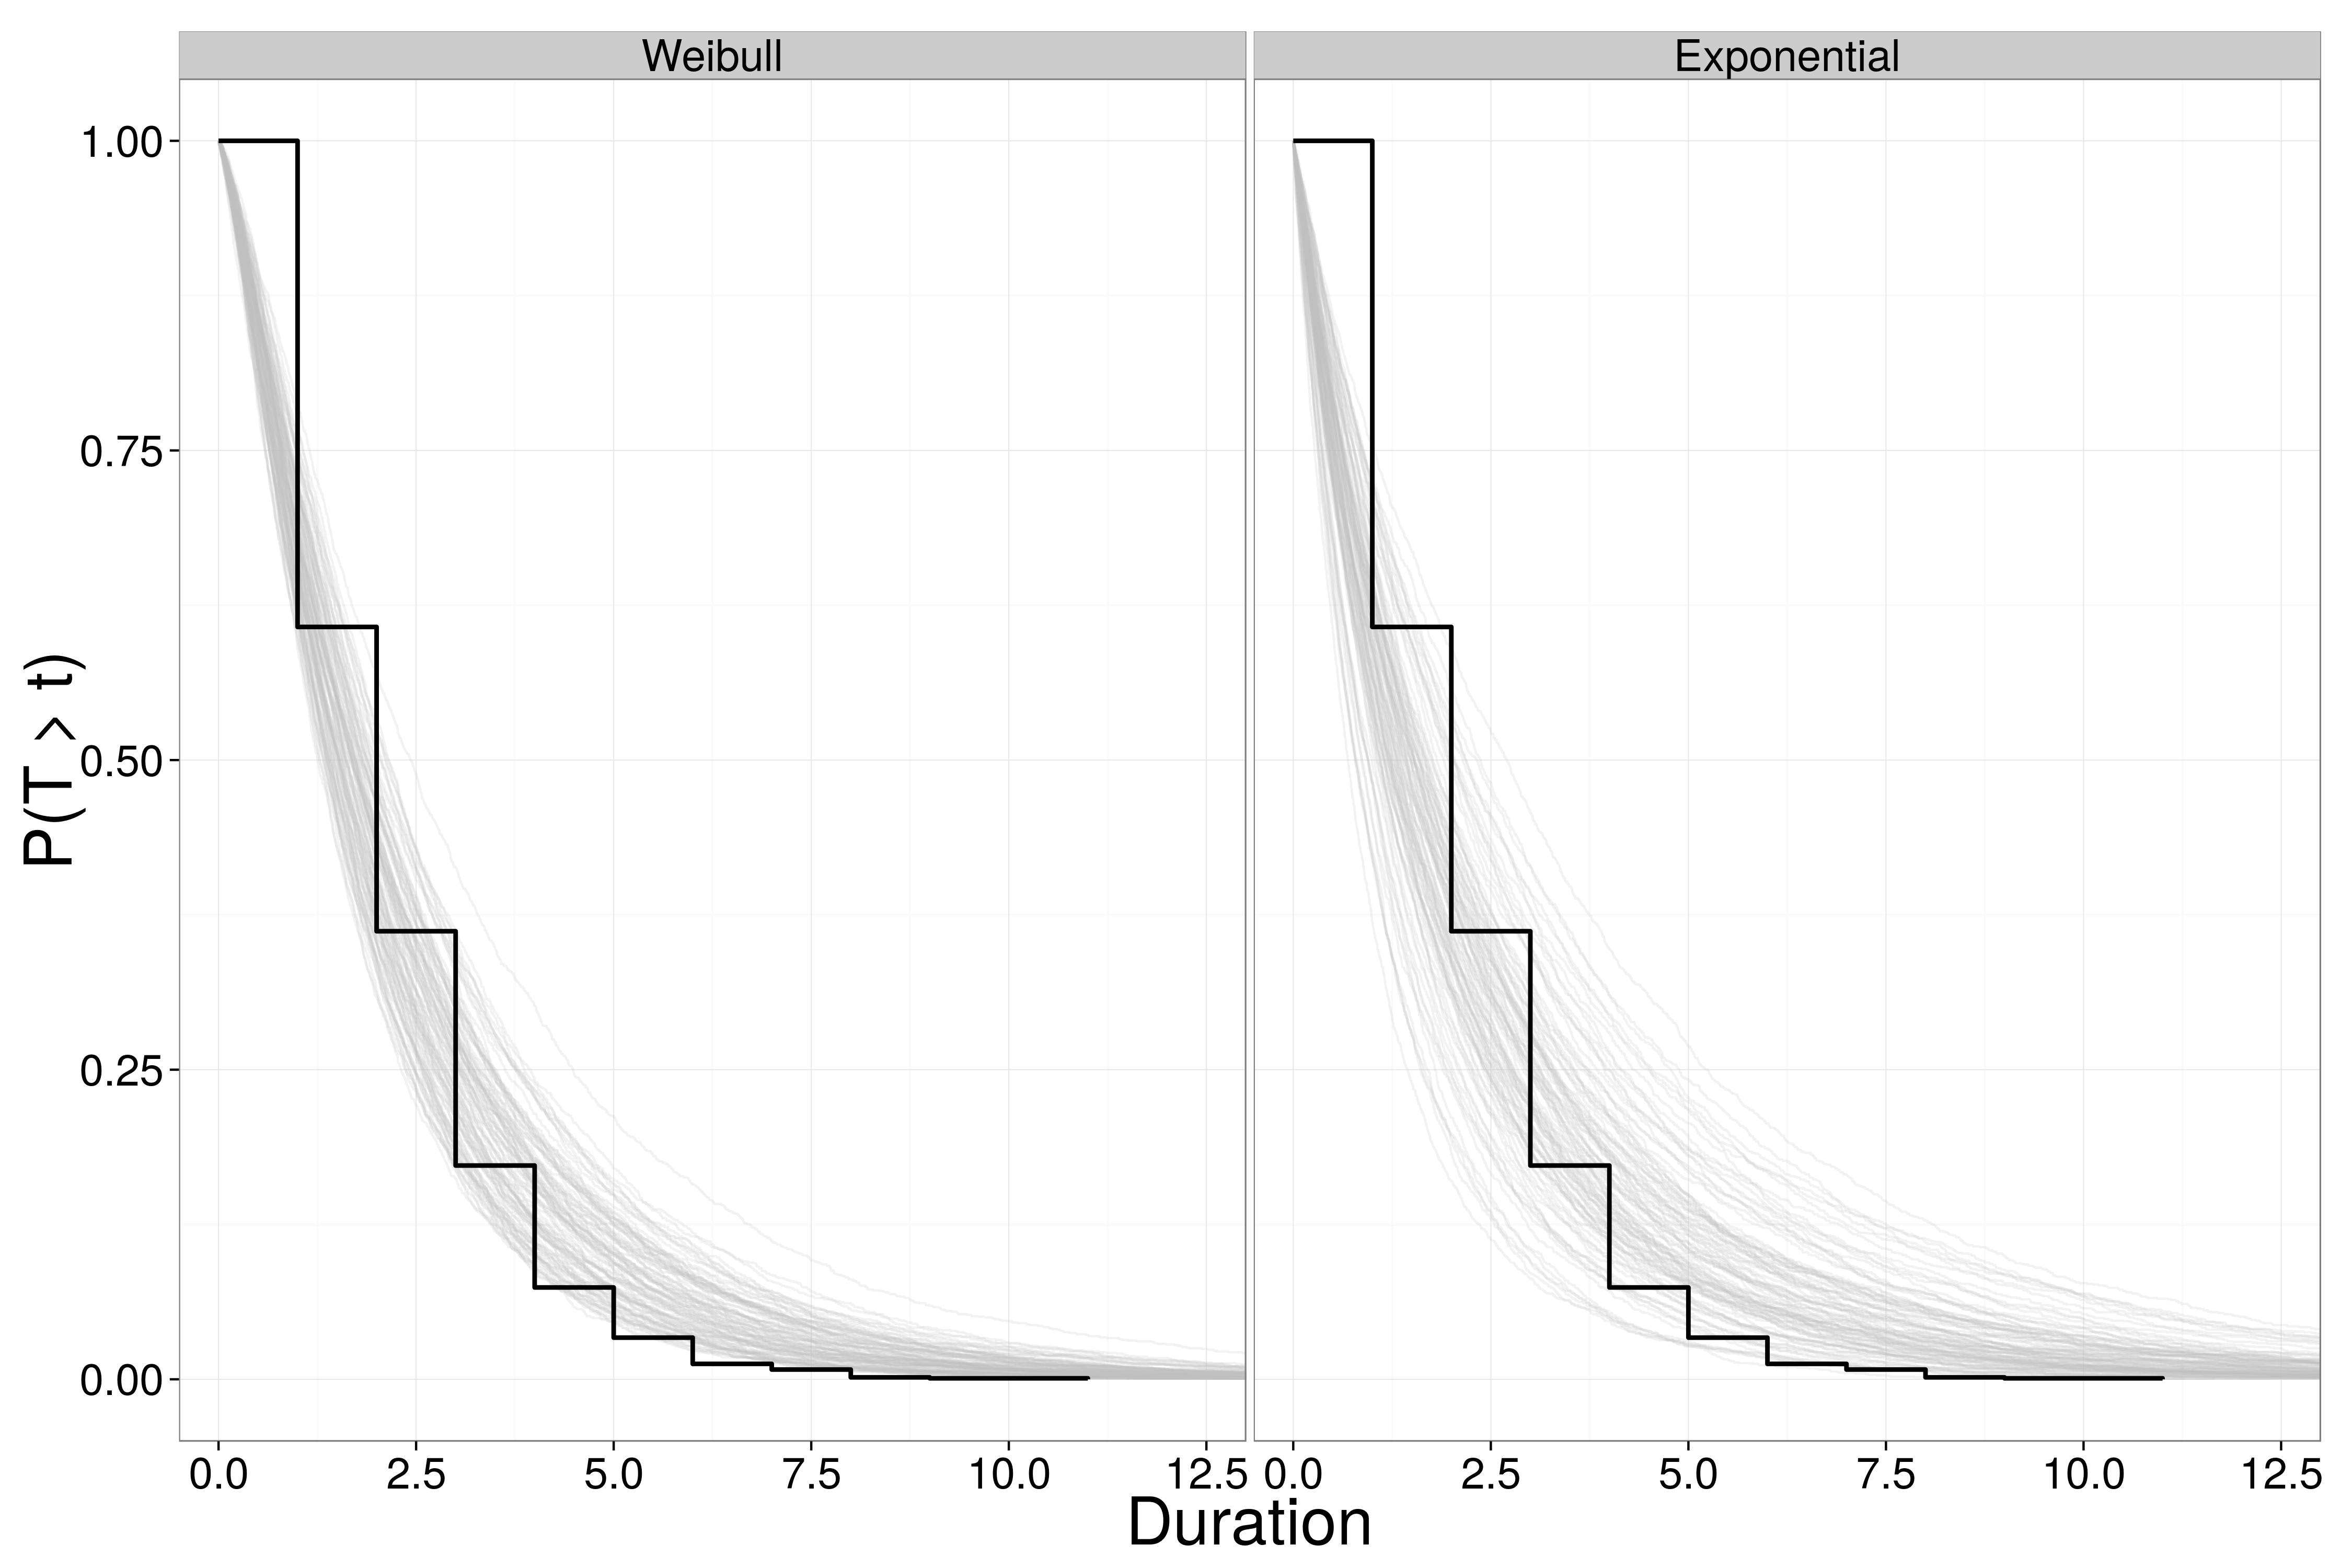
\includegraphics[height = 0.5\textheight, width = \textwidth, keepaspectratio = true]{figure/survival_function}
  \caption{Comparison of K-M estimate of survival function (black) from the observed estimates from 100 simulated data sets using the fitted model (dark grey). Simulated data sets were generated by drawing parameter values randomly from their estimated posteriors and using the observed covariate information to estimate durations for all the observed species. On the left are the results from the full survival model, while on the right are the results from a simplified model where duration follows an exponential distribution and there is no phylogenetic effect.}
  \label{fig:ppc_surv}
\end{figure}


\begin{figure}[ht]
  %\centering
  %\begin{subfigure}[b]{0.4\textwidth}
  %  \caption{}
  %  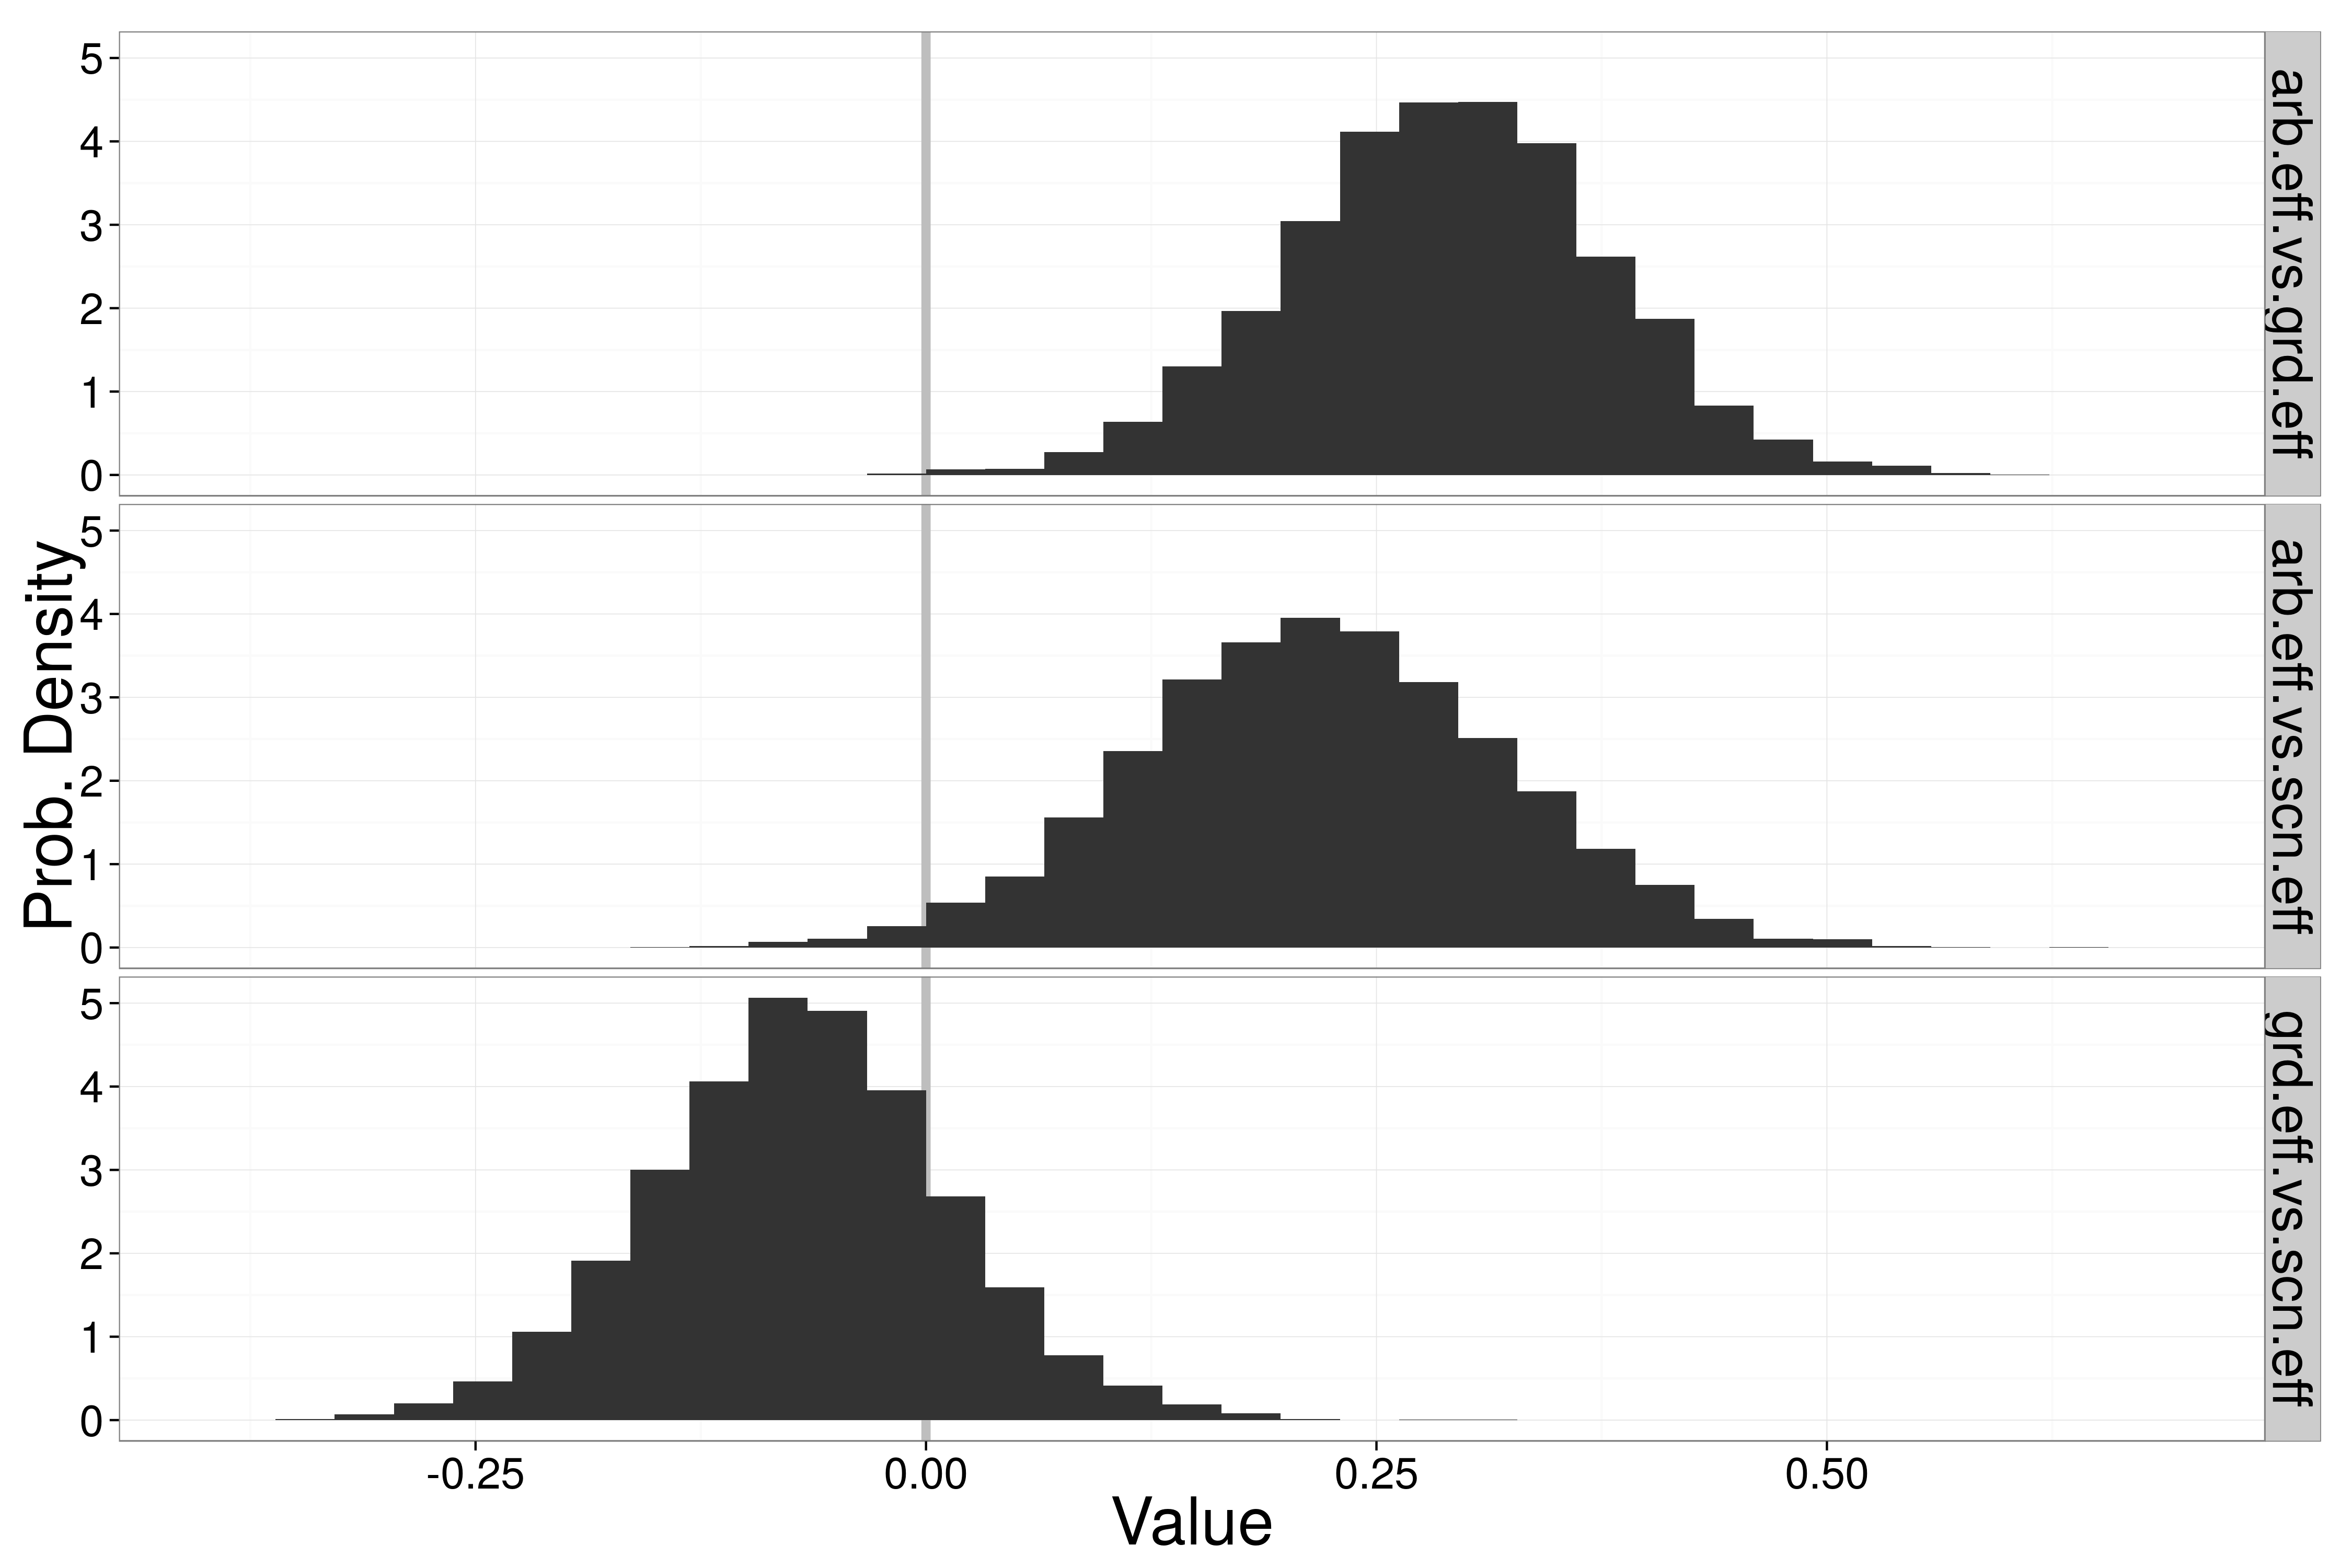
\includegraphics[height = 0.5\textheight, width = \textwidth, keepaspectratio = true]{figure/loco_diff_est}
  %\label{subfig:loco}
  %\end{subfigure}
  %\begin{subfigure}[b]{0.4\textwidth}
  %  \caption{}
  %  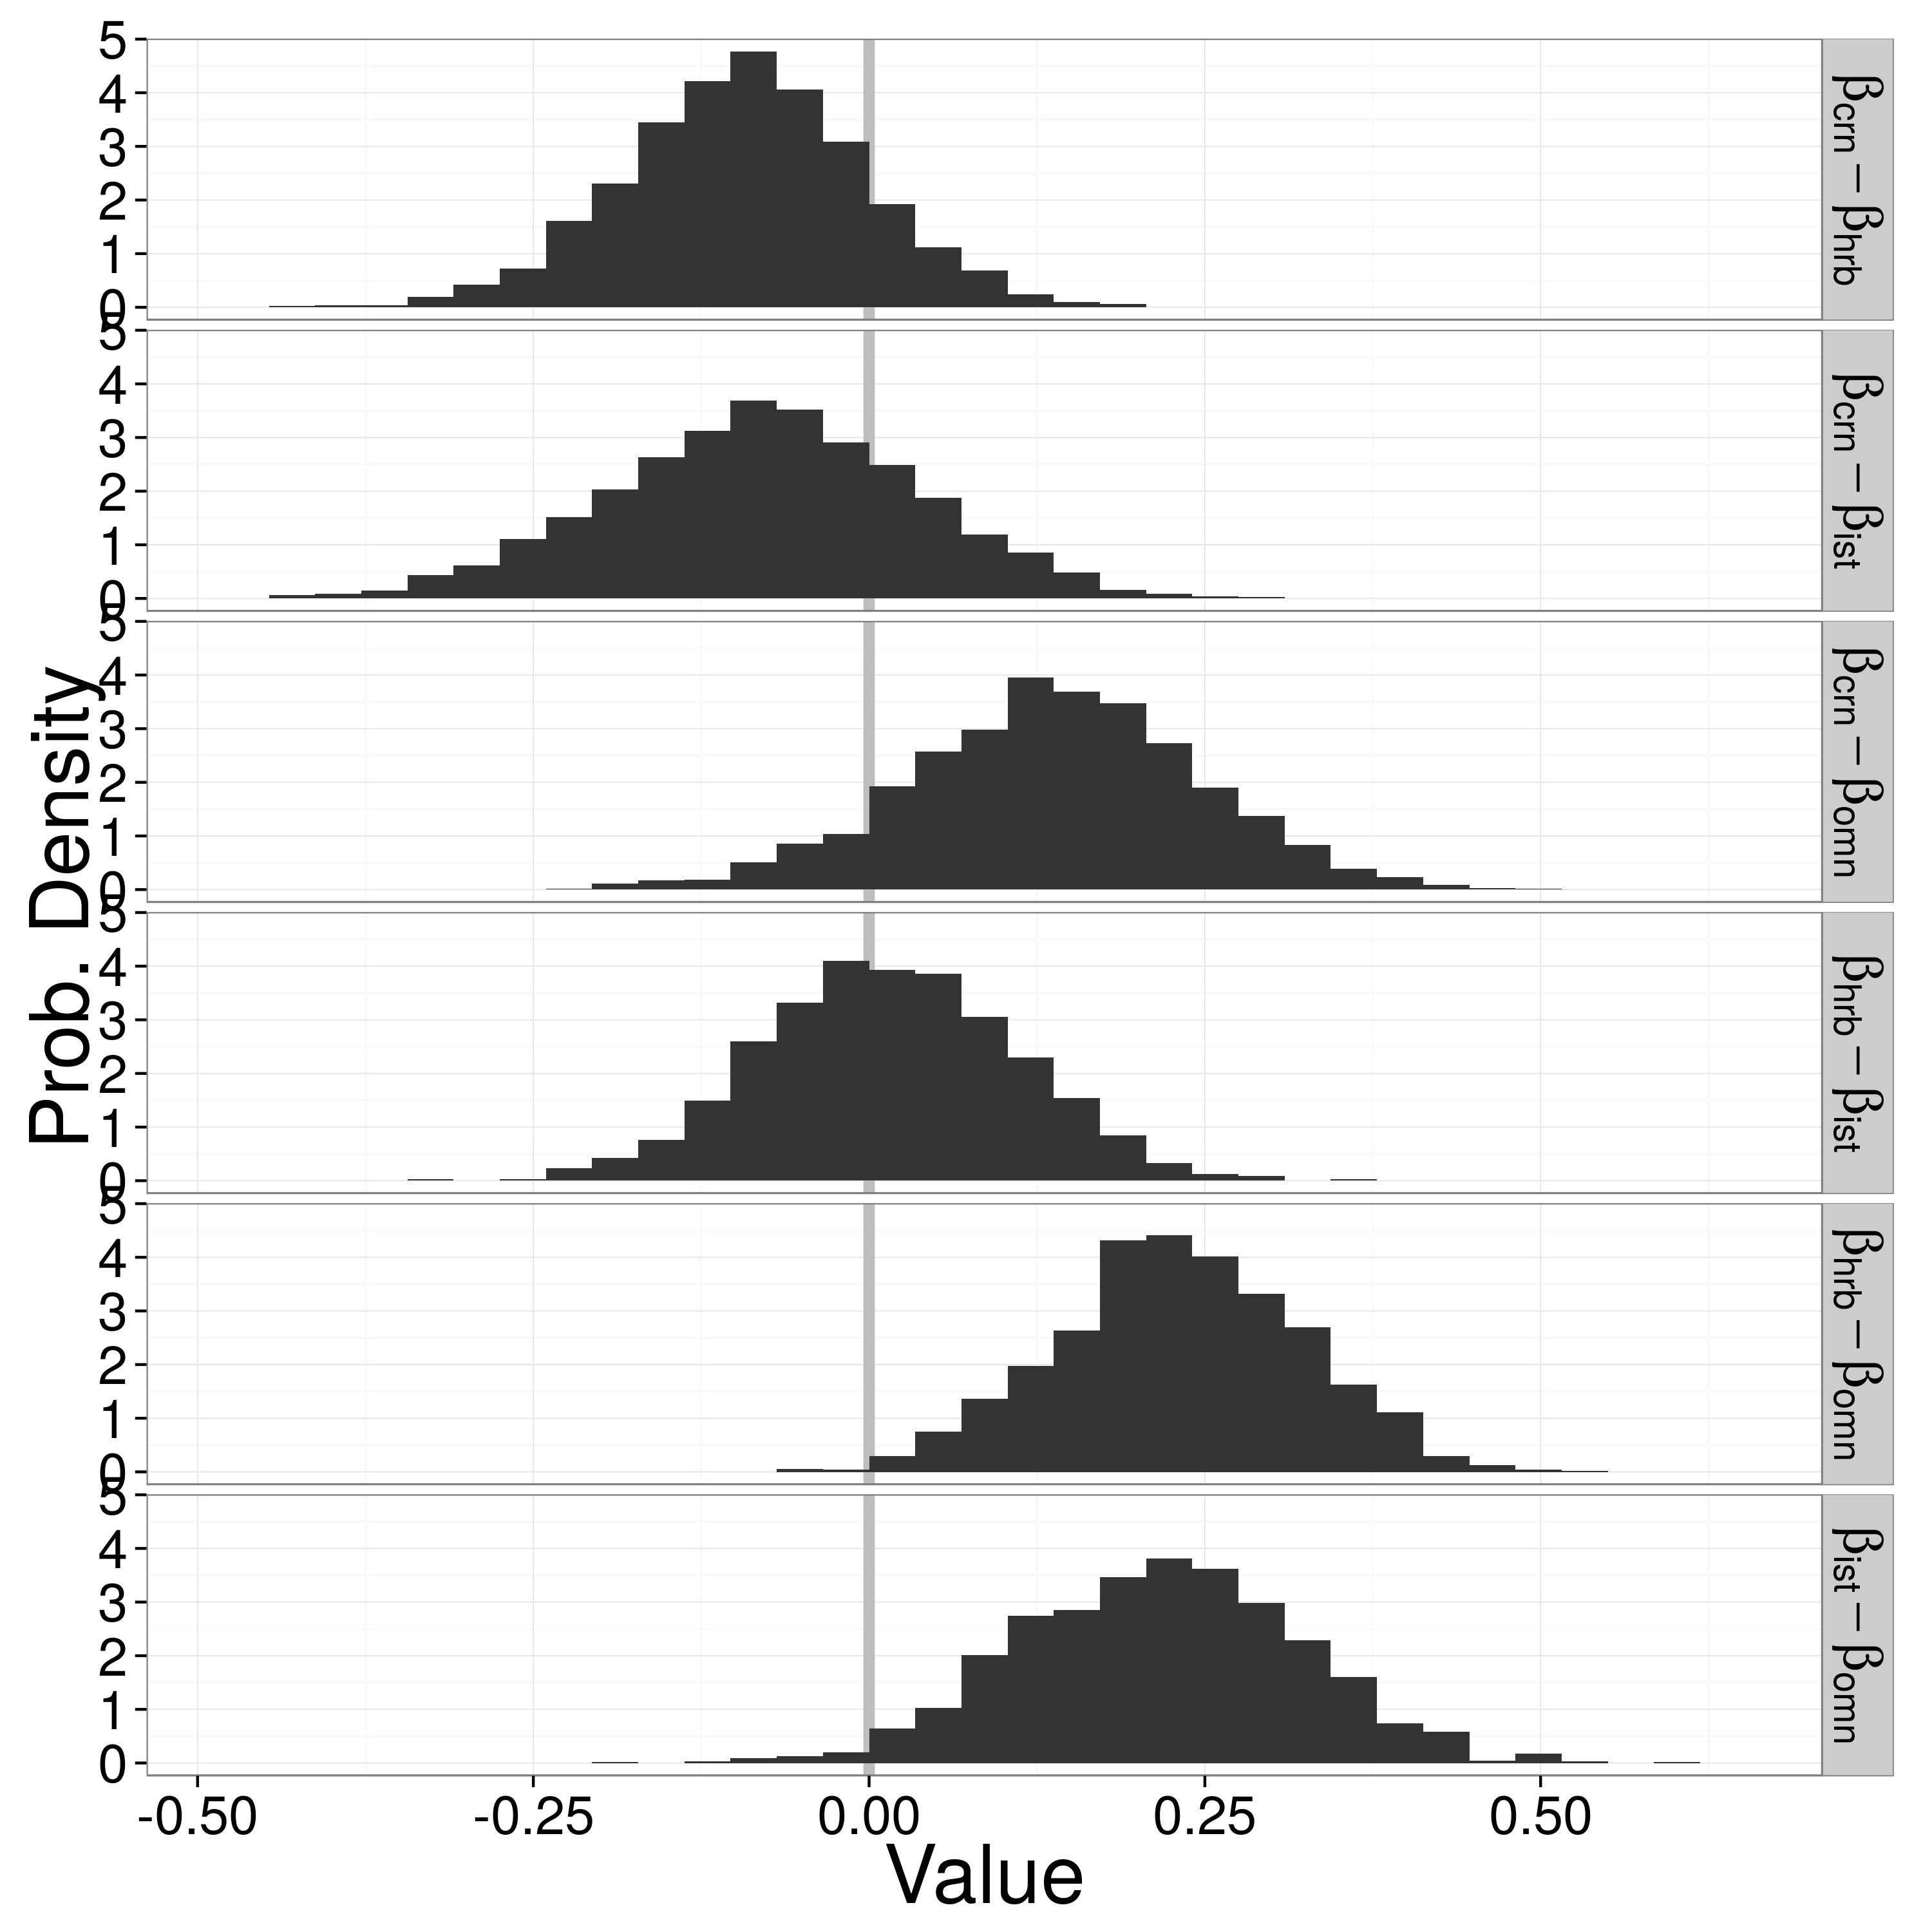
\includegraphics[height = 0.5\textheight, width = \textwidth, keepaspectratio = true]{figure/diet_diff_est}
  %\label{subfig:diet}
  %\end{subfigure}
  \caption{Pairwise differences in effect of the locomotor (\textbf{A}) and dietary categories (\textbf{B}) on expected duration from 1000 samples from the posterior distribution. Comparisons of locomotor categories, from top to bottom (\textbf{A}), are: arboreal versus ground dwelling, arboreal versus scansorial, and ground dwelling versus scansorial. For dietary category, from top to bottom (\textbf{B}): carnivore versus herbivore, carnivore versus insectivore, carnivore versus omnivore, herbivore versus insectivore, herbivore versus omnivore, and insectivore versus omnivore. Values to the left indicate that the first category is expected to have a greater duration than the second, while values to the right indicate that the first category is expected to have a shorter duration.}
  \label{fig:trait_est}
\end{figure}

\begin{figure}[ht]
  %\centering
  %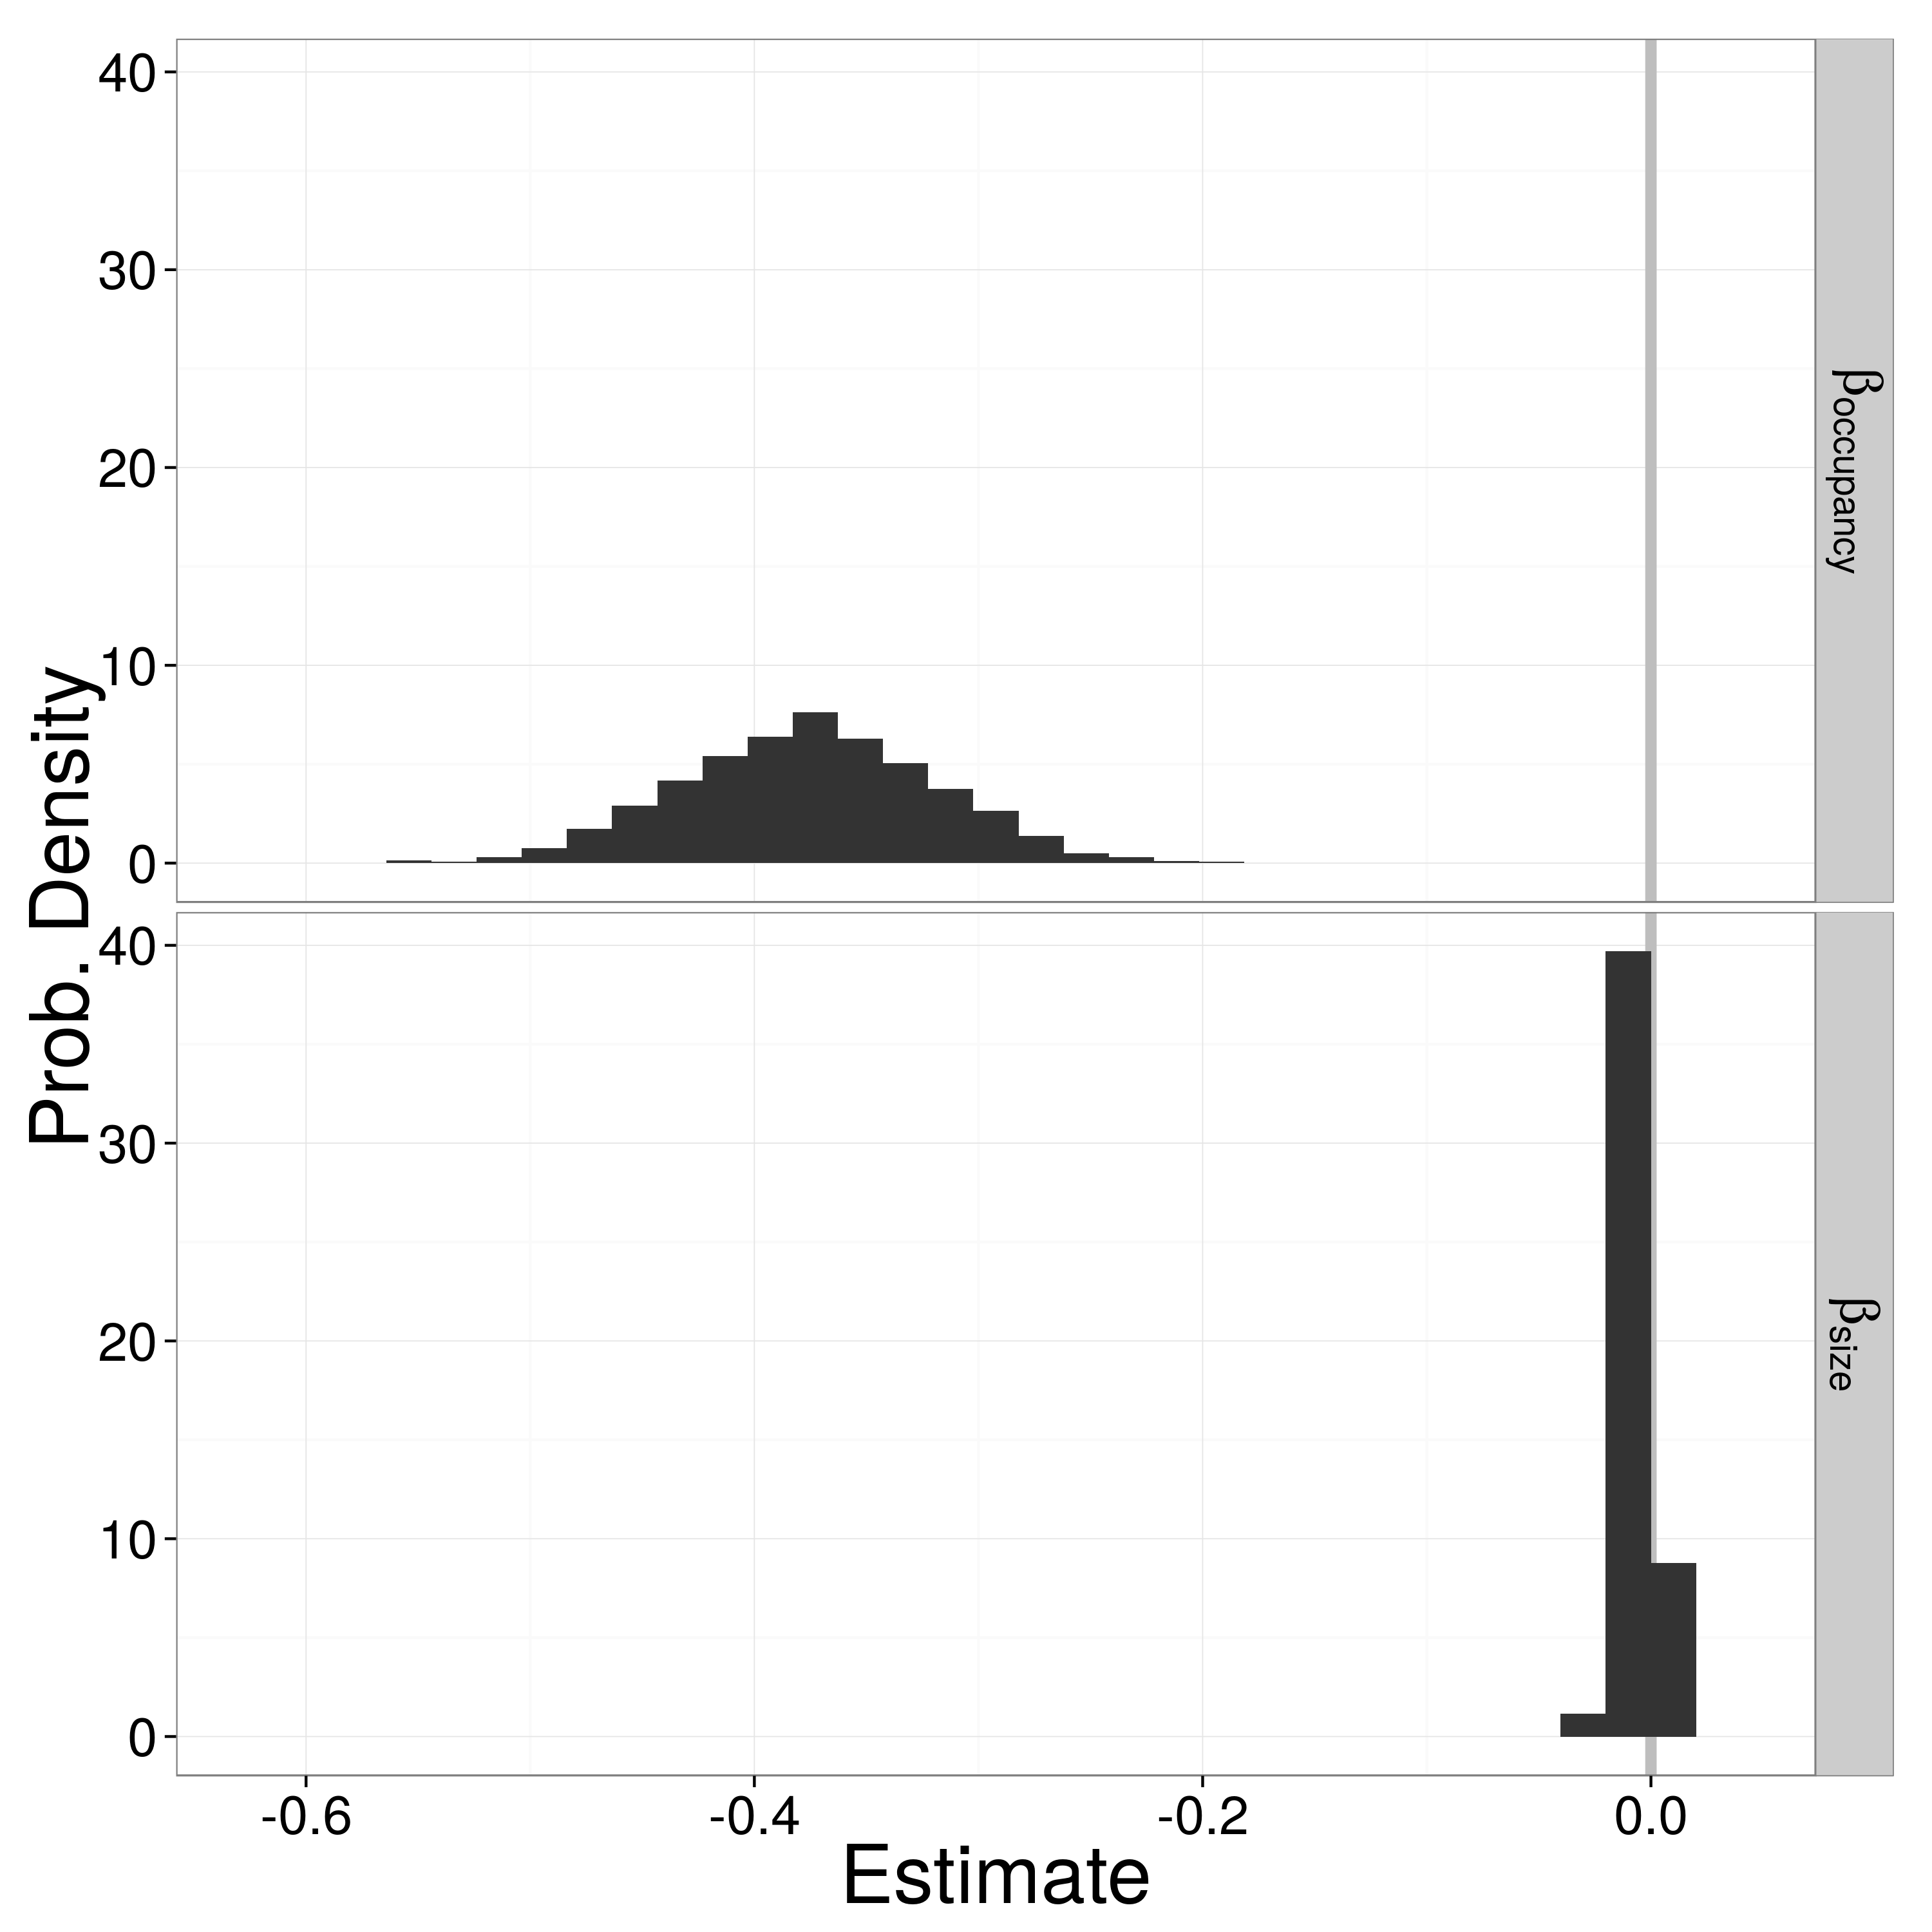
\includegraphics[height = 0.5\textheight, width = \textwidth, keepaspectratio = true]{figure/other_est}
  \caption{Marginal posterior estimates for regression coefficients for the effect of biogeographic occupancy and body size on species expected duration. Posteriors are approximated from 1000 random samples.}
  \label{fig:eff_other}
\end{figure}

\begin{figure}[ht]
  %\centering
  %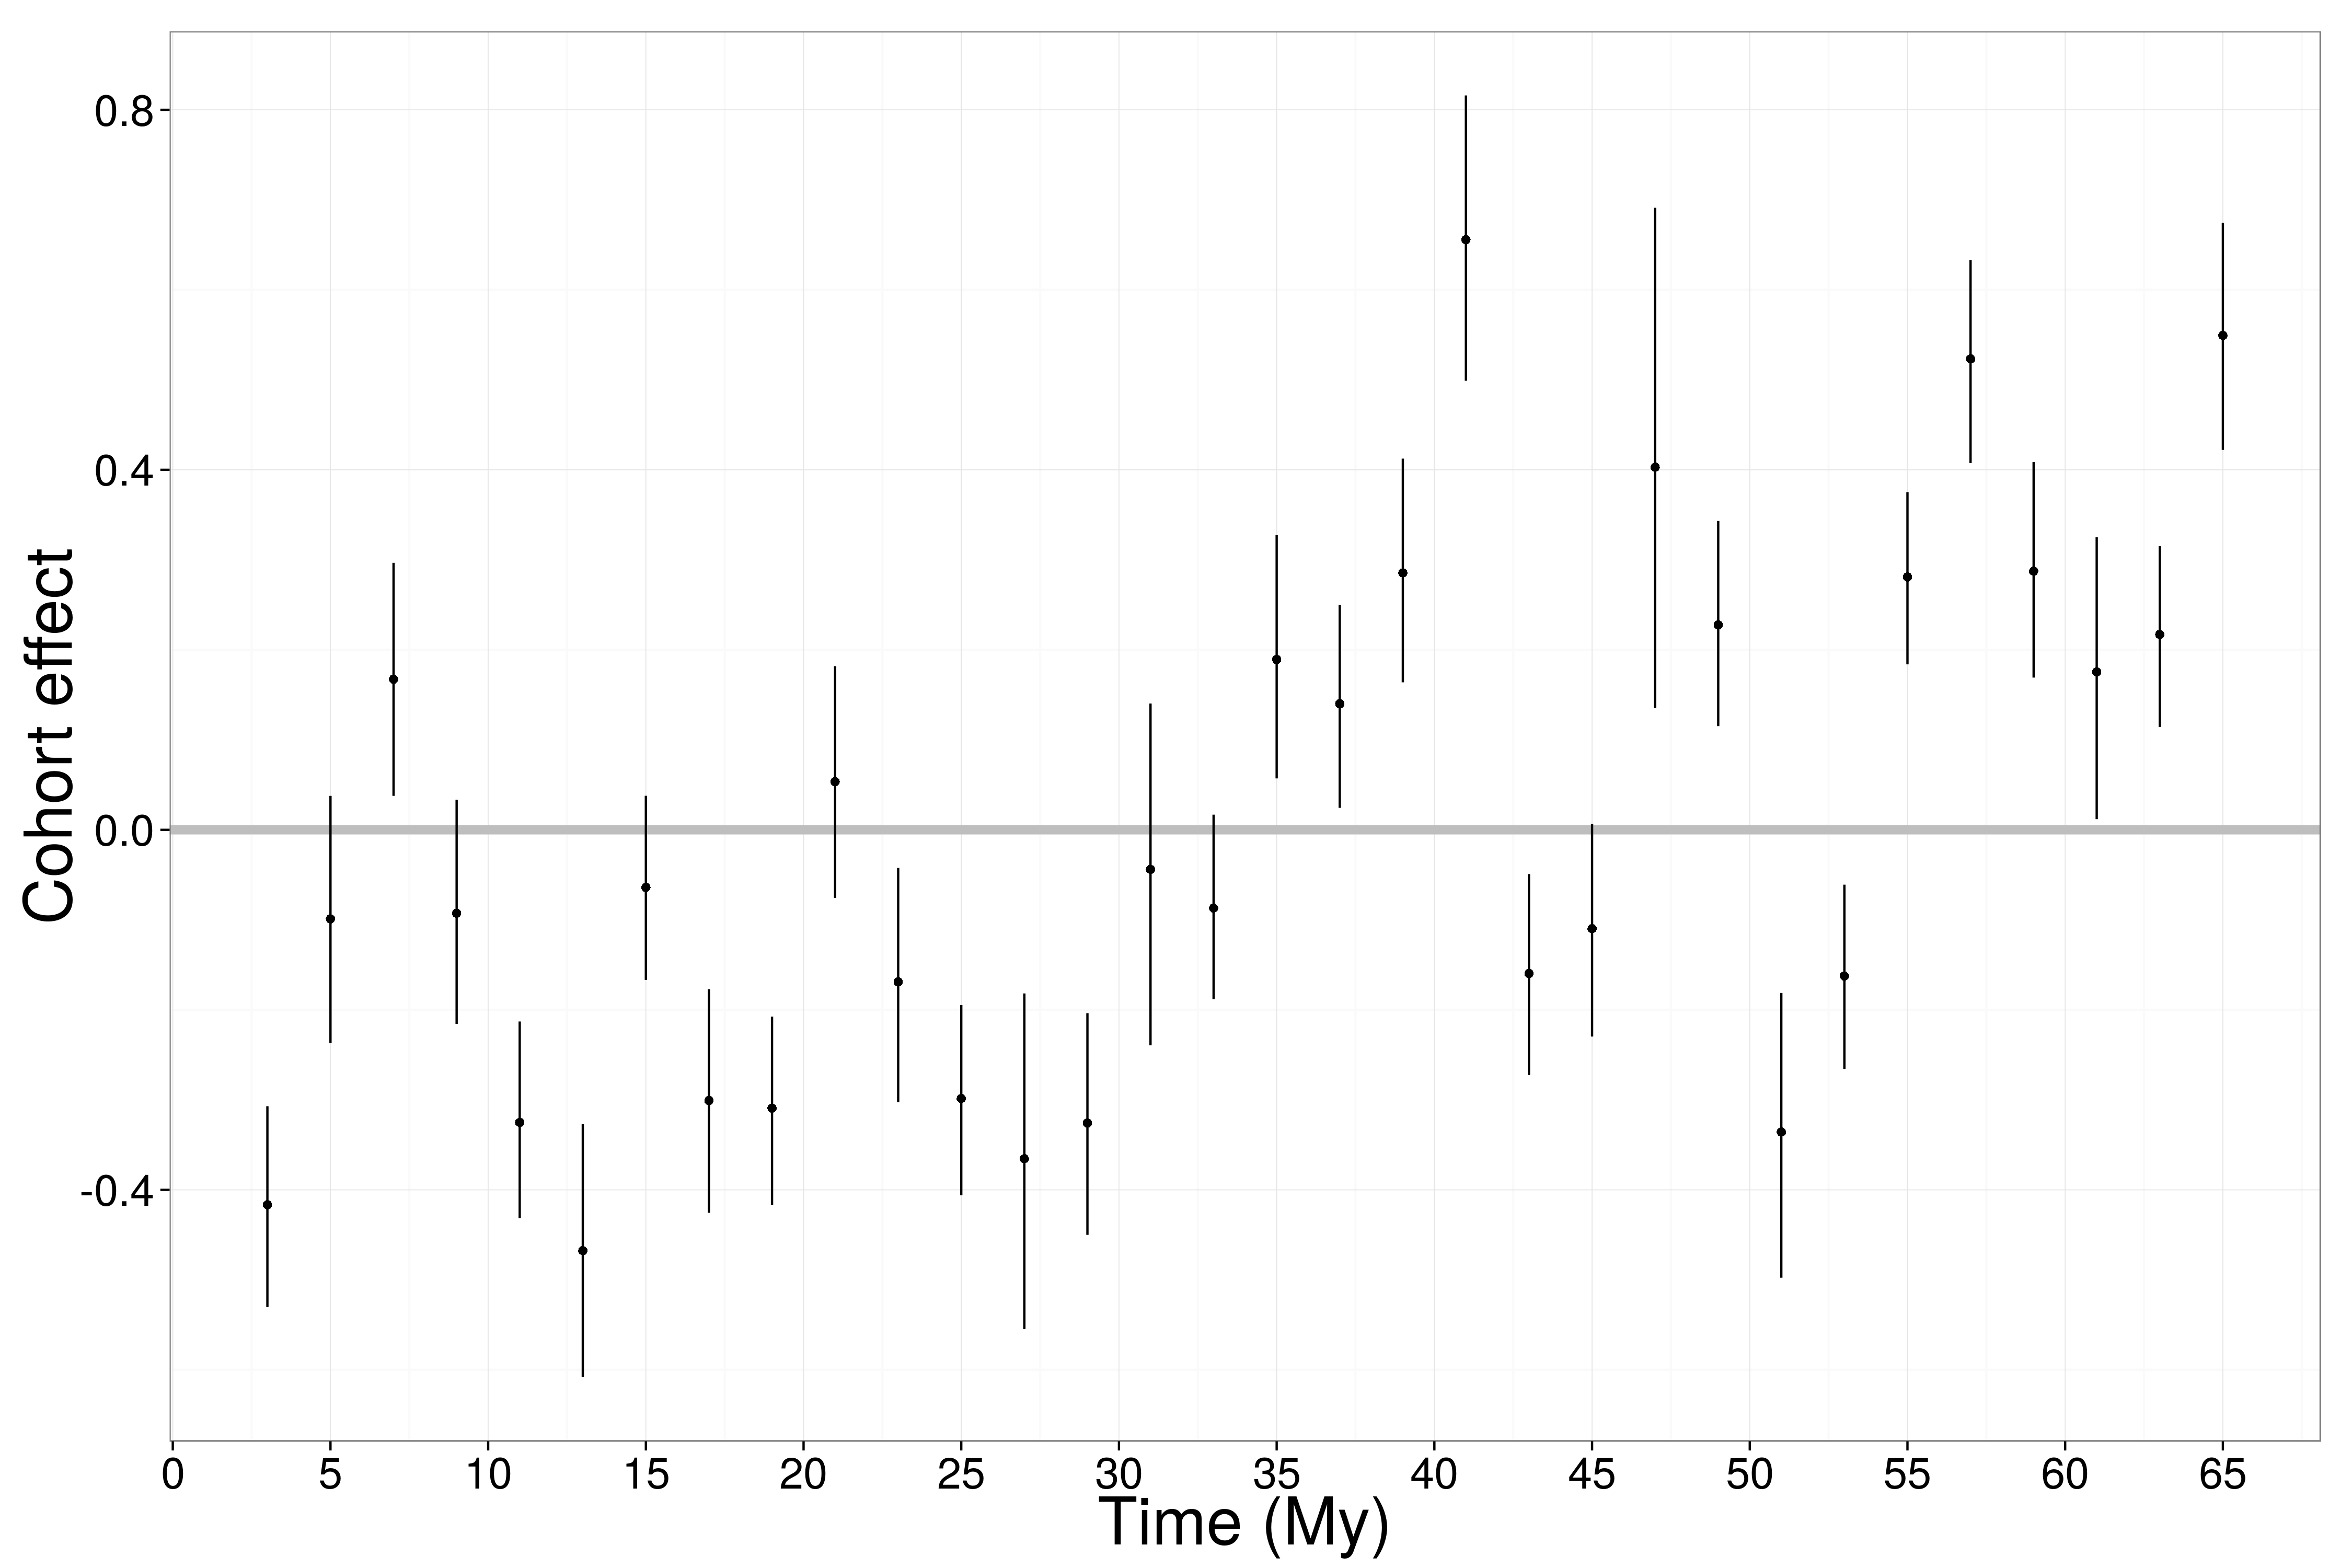
\includegraphics[height = 0.5\textheight, width = \textwidth, keepaspectratio = true]{figure/cohort_est}
  \caption{Summaries of posterior estimates of individual cohort effect depicted as medians and 80\% credible intervals. High values correspond to shorter species durations while lower values correspond to greater species durations compared to the mean duration. Lines are placed at the middle of the 2 My origination cohorts.}
  \label{fig:eff_cohort}
\end{figure}

\begin{figure}[ht]
  %\centering
  %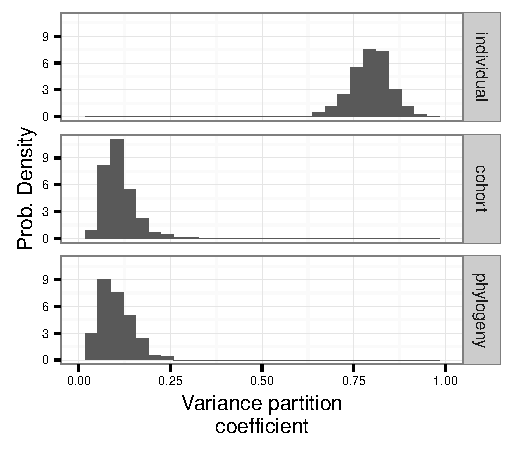
\includegraphics[height = 0.5\textheight, width = \textwidth, keepaspectratio = true]{figure/variance_est}
  \caption{Estimates of the variance partitioning coefficients for the three different sources of variance: species, cohort, and phylogeny. Higher values correspond to greater contribution to total observed variance. Each of the estimates is a distribution of 1000 approximating simulations due to the model's non-normally distributed errors.}
  \label{fig:vpc}
\end{figure}

\end{document}
